\chapter{相关理论和技术}
\section{本章内容}

\section{区块链}
\subsection{区块链简介}
早在1990年,Haber等人首次提出利用链式结构和哈希算法来解决数据的防篡改问题\cite{haber1991time},具体是指新的节点需要包含链上前一个节点的Hash值。哈希算法是一种散列函数,任意长度的数据经过哈希算法的映射都可以得到固定长度的二进制串,即Hash值。对输入数据的任何修改都会导致Hash值完全不同,因此哈希算法可以用来校验原始数据的完整性或是否被篡改。虽然当时并没有使用区块链这个概念,但通常被认为是区块链的最早雏形。直到2008年,中本聪发表的《比特币:一种点对点的电子现金系统》论文\cite{nakamoto2008bitcoin}中提出的比特币项目正是区块链的首个应用,比特币一经问世就以其去中心化、安全性等特性迅速引发了广泛的关注,随后区块链这种技术正式开始流行起来。

随着计算机科学和技术的不断进化,区块链这个概念已经从当初“区块”和“链”组成的数据结构,发展到基于区块链结构实现的分布式数据库技术。
狭义上来说,区块链是由众多包含信息的“区块”依次“连接”组成的链式结构,这种连接通过新的区块中包含前一个区块的唯一Hash值来实现,其基本结构如\autoref{fig:blockchain_data_structure}所示,通过维护这个链式结构,区块链就成为了可以持续增长、且不可篡改的数据记录。
\begin{figure}[htbp]
    \centering
    
\includegraphics[width=.3\linewidth]{pictures/blockchain_data_structure}
    \caption{\label{fig:blockchain_data_structure}区块的基本结构示例}
\end{figure}
广义上来说,区块链代表的是基于区块链结构和点对点(Peer to Peer, P2P)网络实现的分布式数据库技术。所谓点对点网络,即不存在中心服务器为其他节点提供服务,网络中的每一个节点都可以为其他节点提供服务,节点之间可以互相交换信息。比特币项目是第一个区块链应用,在比特币系统中存在一个公共账本,记录了网络中所有的交易记录,这个账本就分布在区块链的一个一个区块上。每个节点都持有一份完整的账本,同时接收网络中的交易信息,并进行记账,满足一定条件后,可以将自己的账本打包成一个区块并链在区块链的后面。

区块链的分布式存储方式与传统的分布式存储体系在两个主要方面有显著的区别:首先,每个区块链节点都会以链式结构保留所有数据的完整副本,而传统的分布式存储系统通常会根据特定规则将数据切分并在多个存储设备上进行备份。其次,区块链中的每个节点都是独立且地位平等的,它们通过共识机制来确保数据的一致性,然而在传统的分布式存储中,数据通常由中心节点同步至其他备份节点。

在区块链系统中,没有任何一个节点能够单独对账本数据进行操作,这极大地降低了由于单一记账实体被操纵或贿赂而导致的数据篡改风险。而且,由于记账节点数量众多,理论上除非所有节点都遭到破坏,否则账本数据将始终保持安全,这在很大程度上确保了账本数据的安全性。

\autoref{fig:blockchain_hierarchy}显示了区块链系统的架构模型。
\begin{figure}[htbp]
    \centering
    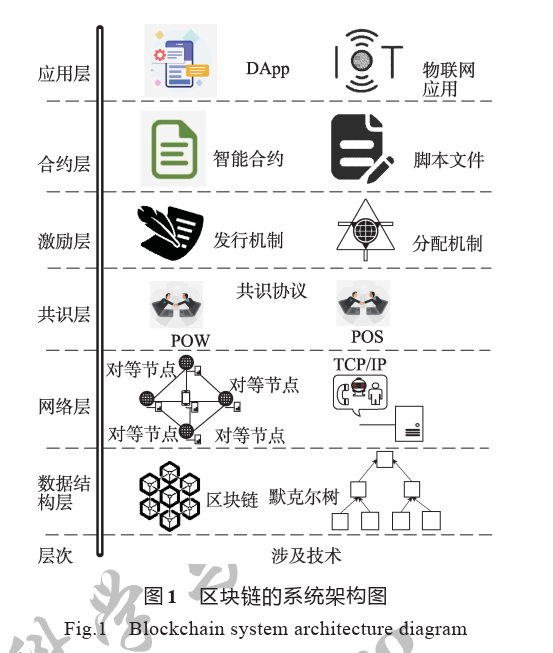
\includegraphics[width=.3\linewidth]{pictures/blockchain_hierarchy}
    \caption{\label{fig:blockchain_hierarchy}区块链系统的架构模型}
\end{figure}
\subsection{区块链中的关键技术}
区块链以其安全性、高度透明和不可篡改的特性,为构建去中心化的多方协同网络提供了可信基础,被普遍认为是一项极具革命性和颠覆性的创新技术,接下来本文简要介绍一下其中的关键技术。
\begin{enumerate}[label=\Alph*., align=left, leftmargin=*]
    \item 去中心化
    
    区块链系统的去中心化特性由P2P网络保证。与P2P网络相对应的是传统的具有中央服务器的C/S网络系统,用户接入网络后,任何与其他用户的交互行为都需要中央服务器进行转发,比如发送邮件、微信聊天、网络转账等,都需要先将请求发送到第三方软件公司的服务器上,后台程序处理这些请求并将数据发送给转账接收方或收信人。P2P网络的工作过程与上述过程截然不同。在P2P网络中,每一个网络节点既是一个用户,也能承担服务器的角色为其他节点提供服务,同时网络中的所有节点都是平等的,没有中心节点,任意两个节点之间都可以互相传输数据。在这个过程中,点对点传输既避免了因中央服务器宕机导致的网络
    \item 一致性
    
    区块链最大的问题之一是在一个由不可信节点组成的网络中达成共识。这个问题类似于拜占庭将军问题\cite{Lamport1982TheBG},有若干支军队包围了一座城市,所有军队必须同时发动进攻才能获得胜利,但有些军队可能会选择撤退,不同军队之间只能通过信使传递消息,但有些信使可能篡改或伪造消息,因此问题就在于如何协调所有军队的进攻时机以获得最大胜利。上述问题说明了在分散、不受信任的环境中达成共识的难度。由于区块链的去中心化性质,它没有中心节点来协调其他节点,因此需要有一套规则让所有节点达成一致,以保证整个网络中只有一条“区块链”,这便是共识机制(Consensus)。工作量证明(Proof of Work,PoW)和权益证明(Proof of Stake,PoS)是最常用的实现节点共识的算法。
    \begin{itemize}
        \item 工作量证明
        
        工作量证明是区块链中最早引入的共识机制之一,也是比特币使用的共识机制。它的基本原理是通过解决数学难题,证明在创建新区块的过程中,进行了一定量的计算工作,这个过程称为挖矿(Mining)。这个数学难题是找到一个前几位为零的哈希值,难点在于用户只能不断尝试不同的输入并验证结果。多个矿工同时尝试解决这个数学难题,竞争成为下一个区块的创建者,第一个成功找到符合条件的哈希值的矿工有权创建新的区块,并将这个区块广播到网络上,其他节点会验证这个区块的有效性,如果验证通过,就接受这个区块,区块链的长度此时就会增加1。尽管工作量证明被广泛应用,但由于矿工需要进行大量的无意义的计算它也有一些缺点,最显著的是能源消耗大。这也导致了对更环保的共识机制的不断探索,如接下来要介绍的权益证明等。
        \item 权益证明
        
        权益证明试图解决工作量证明算法中的能源消耗问题。在权益证明算法中,拥有更多加密货币的用户创建的新区块更容易被接受,这个算法假设拥有更多加密货币的用户越倾向于维护整个网络的稳定\cite{zheng2017overview},这与现实生活中的股份制较为相似,持有股份更多的人拥有更大的话语权。但在实际情况中,这种算法更容易产生垄断情况,即富有的人通过记账获得奖励后会变得更富有,因此也有一些变种形式的权益证明法被提出,如委托权益证明(Delegated Proof of Stake,DPos)。
        \item 委托权益证明
        
        委托权益证明由权益证明法改进而来,其原理是这样的,先根据持有的加密货币数量选出一些代表用户去竞争记账权,每个用户可以进行投票,选出更适合记账的用户代表,如果拥有记账权的用户不称职,就随时有可能被投票出局,这在一定程度上改善了权益证明法的缺点。
    \end{itemize}
    \item 安全性
    
    区块链主要依靠加密技术来保证数据的安全性和防止数据被篡改。前一个区块的数据和哈希值决定了下一个区块的哈希值,倘若区块中的数据被篡改,无论篡改的数据量大小如何,都会导致最终生成的哈希值与原始数据生成的哈希值截然不同。同时,在共识机制的作用下,被篡改的数据不会得到其他节点的承认,除非攻击者能操控整个网络中超半数的节点,而这显然是不可能的。除此之外,密码学中的非对称加密算法也能保障区块链的安全性。非对称加密算法使用一对密钥:公钥和私钥,公钥是公开的,私钥只有用户本人持有。用户可以使用私钥对交易进行签名,其他用户可以使用该用户的公钥对该交易进行验证,这便是数字签名,数字签名确保了交易的真实性和不可抵赖性,因为只有私钥的持有者才能正确地对交易签名。
    
\end{enumerate}

\section{以太坊}
\subsection{以太坊简介}
在比特币项目获得巨大成功后,有一些开发者开始思考能否将区块链技术拓展到更多的应用场景,原因在于比特币项目的本义就是使用数字货币存储价值,其智能合约语言的局限性使得比特币系统难以扩展出其他能力。2013年底,维塔利克·布特林提出了在区块链上运行图灵完备的应用程序的设想,为此他提出了以太坊项目。以太坊也有其专属的电子货币——以太币,除了基本的金融交易,以太坊还支持用户开发部署自己的智能合约,创造各种去中心化应用程序,因此以太坊也被称为“下一代电子货币和去中心化应用平台”。下面简要介绍一下以太坊的主要特点。
\begin{enumerate}[label=\Alph*., align=left, leftmargin=*]
    \item 账户
    
    比特币系统作为分布式记账平台,任何人都可以通过遍历交易历史推断出用户的余额。而以太坊针对此提出了账户的概念,账户可以记录多种类型的信息,如用户的余额、智能合约代码等,以太坊中共有两种类型的账户:外部账户(Externally Owned Account,EOA)和合约账户(Contracts Account)。
    \begin{itemize}
        \item 外部账户
        
        外部账户类似现实世界中的银行账户,是以太币拥有者的账户,记录了用户的余额和发送交易的数量等信息。外部账户可以互相转账,也可以调用合约账户以执行智能合约代码。外部账户与一对密钥绑定,公钥被公开作为账户地址,其他用户可以通过此地址进行转账;私钥由用户本人持有,可以对该外部账户进行完全访问和控制,该账户发送的每个交易都需要使用私钥进行签名,其他账户可以使用公钥进行验证以实现防伪。
        \item 合约账户
        
        合约账户即智能合约账户,主要功能就是存储智能合约代码。用户编写好智能合约代码并部署到以太坊时,合约账户就会被创建。合约账户也可以持有和接收以太币,用于支付合约代码的存储和执行所消耗的网络资源。和外部账户不同的是,合约账户只有公钥没有私钥,它们不能主动发起交易,只能被外部账户调用。
        
    \end{itemize}
    \autoref{fig:ethereum_account}显示了以太坊账户的基本结构。
    \begin{figure}[htbp]
        \centering
        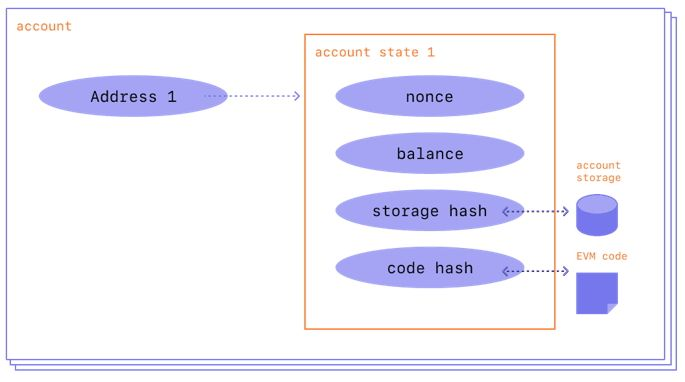
\includegraphics[width=.3\linewidth]{pictures/ethereum_account}
        \caption{\label{fig:ethereum_account}以太坊账户的基本结构}
    \end{figure}
    \item 交易
    
    交易是用户在以太坊网络上交互的主要方式,通过交易,用户可以进行转账、部署或调用合约。需要注意的是,交易只能由外部账户发起,并且在发送交易前,用户需要缴纳一定的手续费,通过以太币方式进行支付,这个费用被称为“Gas”。发起一笔交易需要指定一些关键信息,如交易的发送方和接收方地址、发送的以太币数量,可以消耗的最大Gas数量等。目前以太坊支持三种类型的交易:
    1)转账:将以太币发送到另一个账户,可以是外部账户也可以是合约账户;
    2)部署合约:将编写好的智能合约代码部署到以太坊网络上;
    3)执行合约:使用指定参数调用已部署的智能合约。

    交易是以太坊中的关键技术,它帮助价值在网络中传递,促进了金融交易和去中心化应用的实现。
    \item 去中心化应用
    
    任何人都可以在以太坊上部署自己的去中心化应用(Decentralized App,DApp),去中心化应用与中心化应用相对,前者没有固定的中央服务器,而是借助点对点网络实现分布式存储和计算。去中心化应用由前端和后端构成,前端是用户界面,可以由任何语言编写,用户可以通过它与应用程序进行交互;后端则是部署在区块链上的智能合约,其中定义了应用程序的执行逻辑。去中心化应用依托区块链技术,具有去中心化、开源、自治和透明的特点,可以为用户提供更高的可靠性和安全性,DApp的应用领域也将随着区块链技术的发展而不断扩大。
\end{enumerate}

\subsection{以太坊运行机制}
\section{智能合约}
\subsection{智能合约简介}
智能合约是一种自动执行的计算机程序,可以由高级编程语言(如Solidity)编写,并在预定的条件被触发时自动执行。智能合约的概念最早由密码学家尼克·萨博(Nick Szabo)在1994年提出,但直到2015年以太坊(Ethereum)诞生,智能合约才真正得到实际应用并开始流行起来。以太坊是一个开源的区块链平台,由Vitalik Buterin提出并撰写了白皮书,在以太坊上可以使用智能合约构建去中心化应用程序(DApps)。

智能合约的主要特性是它能够在没有第三方参与的情况下执行合约,这种特性使得智能合约在许多领域都有潜在的应用。例如,在金融交易中,智能合约可以用于自动执行支付;在供应链管理中,智能合约可以自动追踪和验证商品的来源;在房地产交易中,智能合约可以自动完成物业的买卖和转移。
由于区块链的去中心化、透明和不可篡改的特性,一旦智能合约被部署,就无法被修改,这保证了合约的公正性和可信度。

如今智能合约已经成为区块链技术的不可或缺的组成部分,也是推动区块链技术应用的关键因素。正是智能合约的出现,区块链技术的应用才不再局限于数字货币,为实现去中心化的数字社会提供了可能。
\subsection{智能合约漏洞}

\subsection{智能合约运行时崩溃}

% \section{智能合约安全问题}
% \subsection{智能合约运行机制}
% 智能合约作为计算机程序,一般具有开发、编译、部署、调用和销毁等生命周期。


% 如无特殊说明,本文中讨论的智能合约均指由Solidty语言编写并运行在以太坊虚拟机(Ethereum Virtual Machine, EVM)上的智能合约。

% 智能合约作为一段脚本,可以使用多种高级语言进行开发,如Solidity,Serpent,Vyper等,其中针对以太坊的智能合约通常采用Solidity编写,其语法类似于JavaScript.智能合约的编译和解释执行则通过安装在每个以太坊节点上的以太坊虚拟机(EthereumVirtualMachine,EVM)[9]来完成,根据以太坊白皮书,以太坊系统架构如图1所示.每个以太坊节点架构自底向上分别是操作系统、区块链节点客户端、以太坊虚拟机和智能合约脚本.以太坊正是通过运行在不同主机上的以太坊客户端节点之间的通信来完成各种操作.编写好的合约首先通过EVM编译器编译生成一个ABI文件和一个bin文件,其中ABI文件是合约的接口描述,包括了字段名称、字段类型、参数名称、参数返回值等信息,而bin文件是最终运行在虚拟机上的字节码(bytecode),即一段EVM指令集合.合约的部署是将编译后的字节码上传到以太坊区块链平台上,其过程与发送一笔交易类似,发起地址为发布者的地址,目标地址为零,交易数据被替换为合约对应的字节码.在进行交易打包时,将根据发布者的地址和交易序列号通过加密算法重新计算出一个地址作为这个合约的地址,调用者可通过合约地址对合约进行调用.以太坊中存在两类账户:外部账户和合约账户,外部账户由私钥控制,有账户余额,可以触发交易,但没有代码;而合约账户包含不可修改的智能合约代码,有账户余额,但不能主动发起交易,只能在被触发后执行预先编写的逻辑.因此,合约调用也分为两种类型:一种是由外部账户发起的,称为交易调用;另一种则是由一个合约发起对另一个合约的调用,称为消息调用.此外,智能合约还具有自毁操作,这也是唯一能从区块链上将合约代码移除的方式,它需要在合约编写中执行selfdestruct操作,之后合约账户上剩余的以太币(Ether)会被发送给指定目标,其存储的相关状态和代码也会被移除.而所谓以太币就是以太坊中的通用货币,类似于比特币.
% \autoref{fig:smart_contract_execution}显示了智能合约的
% \begin{figure}[htbp]
%     \centering
%     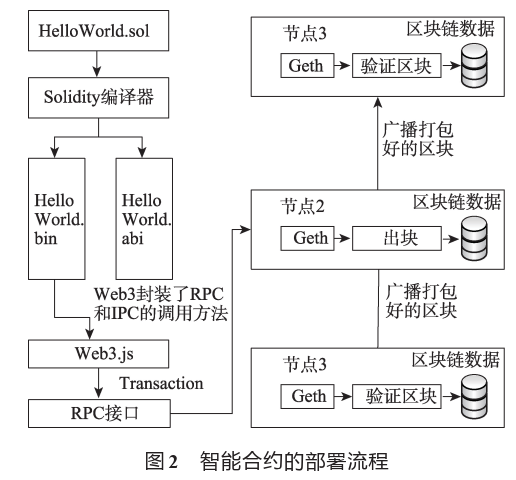
\includegraphics[width=.3\linewidth]{pictures/smart_contract_execution}
%     \caption{\label{fig:smart_contract_execution}区块链系统的架构模型}
% \end{figure}
% 不同于传统的应用程序,智能合约设计了一系列适用于区块链技术的机制[10].gas机制:合约需要矿工的强制执行和证明,因此在打包一项交易时,即将其添加到一个区块上时,为了避免交易中包含大量循环等操作造成节点资源的浪费,合约需先行向矿工支付一笔费用(gas).在以太坊执行一份合约需要根据内部制定的规则消耗一定量的gas,如果交易执行后,提前支付的gas还有剩余,则原路返还;如果没有执行结束gas就被耗尽,则会触发一个outGofGgas异常,当前合约程序的所有执行状态都会被回滚,但是因为矿工为了执行相应计算已经付出了算力,所以已经消耗的gas不会被退回.委托调用机制:合约可以通过消息调用的机制来调用其他合约,委托调用(delegatecall)就是一种特殊类型的消息调用.它和普通call指令的区别在于,普通call指令的行为是跳转到被调用合约,并在该合约中执行完相应代码再返回执行后续代码,对于调用发起者的上下文无影响;而委托调用则相当于把被调用合约中的一段代码拷贝到调用发起者合约的上下文环境中执行,修改调用发起者的信息.异常传递机制:智能合约的函数调用方式分为内部调用和外部调用,内部函数调用指直接调用当前合约或者父合约的内部函数,这些函数调用在EVM中会被直接转换为简单的跳转指令;而外部函数调用指对于指定地址的外部合约函数的调用,需要靠消息调用完成[10].其中外部调用中的一些低级调用,如call,callcode,delegatecall在执行中如果出错并抛出异常,该异常不会沿着函数调用栈被传递,而是只能获取一个布尔值来表示成功或者失败.此外,一些转账函数,如张潆藜,等:以太坊Solidity智能合约漏洞检测方法综述53call,value,send等,当发生转账异常时,也仅返回一个布尔值而不是回滚这个操作.
% \subsection{智能合约漏洞及检测技术}
% 本节对当前典型的智能合约漏洞类型进行总结,并在详细介绍其原理及利用方式后,给出一些相应的防范措施.根据Atzei等[11]的一份调查报告,智能合约的安全漏洞可以按照高级语言Solidity、EVM和区块链3个层面进行分类.高级语言Solidity层面的漏洞主要为语言自身设计的缺陷以及开发者在开发过程中引入的错误;EVM层面的安全威胁主要由以太坊智能合约字节码规范和运行机制本身的一些缺陷带来;区块链层面的问题由区块链本身的很多特性所致.具体如表1所列.
% (1)整数类型错误.整数类型错误主要包含算数错误、截断错误和符号错误.算数错误包括整数溢出[12]、除数为零和模数为零这3种错误.与其他计算机程序设计语言一样,SoGlidity规定使用几种固定的长度表示一定范围内的整数,一旦整数运算结果超出这个范围就会发生整数溢出.攻击者可以利用该类漏洞跳过某些条件判断或者篡改数据,例如著名的BEC漏洞事件就是由于合约在转账过程中发生了整数溢出,从而导致巨额的代币蒸发[13].而使用提供安全检查的SafeGMath[14]数学计算库可以有效避免溢出漏洞.在EVM和旧版本Solidity中,除数为零和模数为零会导致运算结果为0,并且不会触发异常.截断错误指将一个整数类型数据转换为宽度更短的整数类型数据导致的精度丢失;符号错误指将一个有符号整数类型数据转换为相同宽度的无符号整数类型数据.(2)未校验返回值.以太坊Solidity语言的函数调用和其他高级语言一样,一般都会设置返回值,但是对send,call,delegatecall等低级别函数调用失败时不会引起事务回滚操作,只是在返回值中表示出现了异常.攻击者可以通过故意发送失败的操作来使程序执行与预期设定不同,从而造成智能合约状态混乱.开发者在开发合约时可以通过对低级别函数调用的返回值校验来确定调用是否成功,从而确保合约能以预先设定的逻辑执行.(3)权限控制问题.Solidity中可以使用4种说明符设置函数和状态变量的可见性,分别为external,internal,public和private.未声明可见性的函数被默认为public,即该函数不仅允许内部调用,还可作为合约对外接口被外部合约调用.如果一些涉及转账等敏感操作的函数没有声明可见性,就会存在被攻击者利用的风险.(4)拒绝服务.拒绝服务(DenialGofGService,DoS)一般指不可恢复的恶意操作或者可控制的无限资源消耗.针对以太坊合约的DoS攻击会导致以太币和gas被大量消耗,更有甚者会导致永久性地无法使用合约.2016年的以太坊游戏TheKingoftheEtherThrone,攻击者利用了外部函数调用的漏洞,通过UnexpectedRevert发动DoS攻击,导致该游戏运营出现重大问题[15].(5)资产冻结.由于合约的不可篡改性,如果开发者在进行智能合约开发时仅设置了接收以太币的功能,但没有设置任何允许以太币转出的操作,或由于某些原因使得以太币无法转出,就会造成合约内的资产被永久冻结.(6)重入漏洞.虽然以太坊智能合约的执行是一个具有原子性和顺序性的事务操作,但是用户在调用智能合约时,如果在被调用合约中没有找到被调用的函数或者该合约只接收到以太币而没有其他任何消息时,就会调用回退函数fallGback.攻击者可以通过构造特殊的回退函数来攻击存在重入漏洞的智能合约,例如回退函数中包含重新调用被攻击合约中向攻击者转账的函数,从而通过递归调用耗尽被攻击合约的资产.导致以太坊硬分叉(ETH/ETC)的著名的事件TheDAO就与重入漏洞有关.可以采取如下措施规避潜在的重入漏洞:先保证改变状态变量的逻辑发生后,再允许以太币从合约中转出;或将以太币发送至外部合约时,使用内置的transfer函数代替call,send函数,实现安全的转币操作.(7)短地址攻击.短地址攻击漏洞是一种因未校验用户输入而导致的漏洞,攻击者利用虚拟机的自动补全机制,构造末尾为零的地址进行合约调用,并在传入参数时故意将地址address末尾的零省去,此时虚拟机会取发送代币的金额amount高位的0对地址补全,同时将amount低位补0,这样就等效于amount左移翻倍,导致转移的代币数量超出了原来的设定.通过严格检查用户输入并拒绝接受畸形地址,可以有效避免短地址攻击.(8)代码注入.代码注入漏洞由以太坊的委托调用机制引入.委托调用机制中使用的delegatecall指令允许合约在自己的上下文执行其他合约的代码片段.攻击者可以利用该漏洞向合约注入修改合约中重要状态变量等恶意操作的代码.(9)交易顺序依赖漏洞.一笔交易被传播出去并被矿工认同写入一个区块内需要一定的时间,因此打包在区块中的交易顺序与交易生成的顺序可以不同.攻击者可通过监视网络上依赖于交易顺序的合约并发出自己的交易来改变当前的54ComputerScience计算机科学Vol.49,No.3,Mar.2022合约状态,从而获益.例如,攻击者可以提交一个悬赏合约,允许用户通过提交难题的答案从该合约获得丰厚的奖励,攻击者可以在提交完悬赏合约后持续监听网络,若有人提交了答案且此时提交答案的交易还未被确认,则攻击者可以立刻发起一个将奖金降低到无限接近于0的交易并提供较高的gas,使自己的交易先被矿工处理,这样攻击者支付很少的奖金就能获得问题的答案.(10)时间戳依赖漏洞.在智能合约中可以使用区块时间戳作为条件判断依据,这对普通的攻击者来说没有什么利用价值,但是对于可以在一定范围内操纵时间戳的矿工来说,可以通过构造恶意的时间戳来绕过相关的判定条件.(11)可预测的随机处理.合约开发者编写随机数生成函数时,有时会利用时间戳(block.timestamp)、区块号(block.number)等与区块有关的一些参数产生随机数,但是区块链上的上述数据都是公开的,这使得生成的随机数是可预测的,从而可能会被攻击者利用.